\documentclass[a4paper,11pt]{article}

\usepackage[english]{babel}
\usepackage[utf8]{inputenc}
\usepackage{graphicx}
\usepackage{caption}
\usepackage{subcaption}
\usepackage[T1]{fontenc}
\usepackage{setspace}
\usepackage{geometry}
\usepackage{titling}
\usepackage{float}
\usepackage{comment}
\usepackage[backend=biber]{biblatex}
\addbibresource{refs.bib}
\usepackage{lipsum}
\usepackage{tabularx,booktabs}
\newcolumntype{C}{>{\centering\arraybackslash}X} % centered version of "X" type
\setlength{\extrarowheight}{1pt}
\usepackage[compact]{titlesec}
\titlespacing*{\title}{0pt}{*1}{*1}
%\usepackage{savetrees}
 \geometry{
 a4paper,
 total={170mm,257mm},
 left=20mm,
 top=20mm,
 right=20mm,
 bottom=20mm,
 }
\title{\normalsize\textbf{Fault Tolerance Capabilities of Three, Four and Six Phase Configurations of a 24 Slot Modular PMSM}}
\date{}
\titlespacing\section{0pt}{11pt plus 4pt minus 2pt}{0pt plus 2pt minus 2pt}
\titlespacing\subsection{0pt}{11pt plus 4pt minus 2pt}{0pt plus 2pt minus 2pt}
\titlespacing\subsubsection{0pt}{11pt plus 4pt minus 2pt}{0pt plus 2pt minus 2pt}
\begin{document}
\vspace{-45mm}
\maketitle
\vspace{-23mm}
\textit{\normalsize\textbf{Abstract:}}
\textit{Integrated Modular Motor Drive (IMMD) is the concept of integrating power electronics, electric motor and other passive components of a drive to obtain a more compact system compared to conventional motor drives. In this study, fault tolerance and redundancy capabilities of different phase and winding configurations of an IMMD system is investigated. This is possible by manipulating gate drive signals of the inverter and end winding connections, without making any changes on the stator side of the electric machine. Three, four, symmetric and asymmetric six-phase topologies are described. Control strategies and redundancy possibilities of these different topologies under an open circuit fault condition are examined in MATLAB/Simulink environment and validated with Finite Element Analysis (FEA) software ANSYS/Maxwell. }

\section{\normalsize\textbf{Introduction}}
With the developments in safety-critical industrial applications, fault tolerance, reliability and redundancy of electric motor drive systems have become more important. As described explicitly in \cite{bible}, fault tolerance of a drive is basically the drive's ability of maintaining its operation within the boundaries, in a possible failure occurance. (...)

\section{\normalsize\textbf{Design Specifications of IMMD System}}
IMMD structure proposes placing the electric machine and power electronics into a single housing especially for higher power density and compactness considerations \cite{immd-bible}. There are several types for this integration \cite{difftopology1}\cite{difftopology2}. In this study, power converter and control circuits are placed on the stator back iron \cite{mesutto}. \\
For the machine topology, fractional slot concentrated winding (FSCW) permanent magnet synchronous motor (PMSM) is more suitable due to high power density and high efficiency advantages. Furthermore, complete (electric and physical) isolation of phases and achieving higher number of phases in FSCW increases the fault tolerance capability of the machine \cite{fscw}. Besides, aforementioned integration configuration of drive unit onto the FSCW machine provides modularity for both machine and driver side, which brings redundant operation opportunity. (...)

\begin{table*}[ht!]
\centering
 \caption{Design Specifications of IMMD}
\label{kd}
\begin{tabularx}{0.5\textwidth}{@{}l*{10}{C}c@{}}

\toprule
Specification  &  Value \\ 
\midrule
Rated Output Power & 8 kW \\ 
Speed & 600 rpm \\ 
Number of Slots ($Q_s$) & 24 \\
Number of Poles (2p) & 20 \\
Stator Outer Diameter & 270 mm \\
Stack Length & 135 mm \\
Inverter Input Voltage (Per Module) & 270 Vdc \\

\bottomrule
\end{tabularx}
\end{table*}

\begin{figure}[ht!]
    \centering
    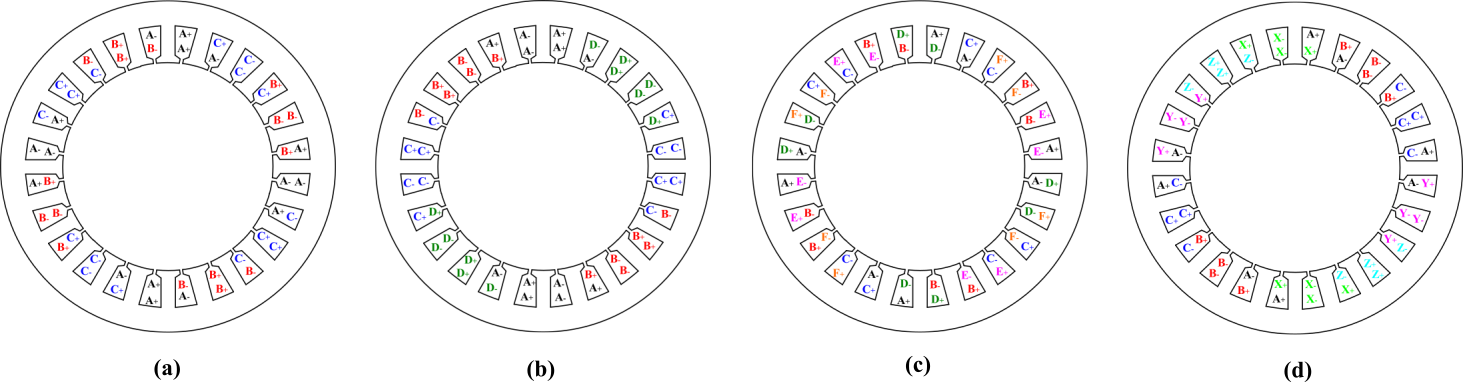
\includegraphics{windings.png}
    \caption{8 kW IMMD System: (a) 24 Slot Stator (b) Heatsink and Driver of a Module (c) Cross-sectional View of Overall System}
    \label{fig:immd}
\end{figure}

\section{\normalsize\textbf{Three, Four and Six-Phase Winding Configurations}}
In a single phase fault condition, a three-phase machine is unable to operate as the machine cannot produce rotating MMF. For that reason, three-phase machines with a redundant phase leg or multiphase machines are more suitable for fault tolerant applications. %\cite{kaynak ver reis}
In this section, different configuration possibilities are to be evaluated. As the stator slot number ($Q_s$) is 24, three, four and six phase topologies are suitable to compare.\\
% Geliştir buraları, şimdilik madde madde
Four phase has high number of harmonics and has very poor winding factor.\\
Symmetric six phase and three phase has suitable winding factor and lower mmf harmonics.
Asymmetric six phase nearly eliminates all sub-harmonics, but due to its winding configuration, one of the phase inductances is expected to be lower than the others.

\begin{figure}[ht!]
    \centering
    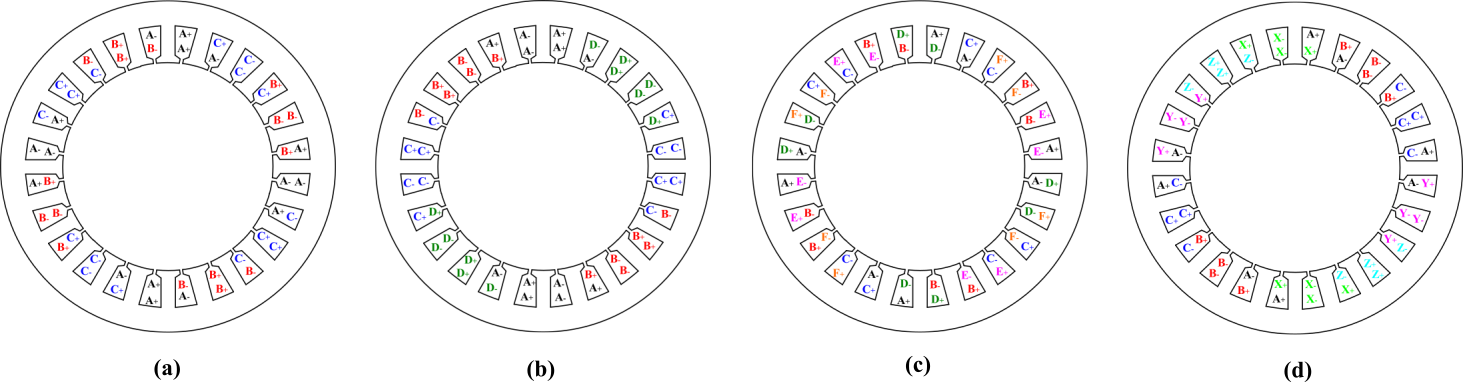
\includegraphics{windings.png}
    \caption{Winding Diagrams: (a) Three-Phase Four Modules (b) Four-Phase Two Modules (c) Symmetric Six-Phase Two Modules (d) Asymmetric Six-Phase Two Modules  }
    \label{fig:winding}
\end{figure}

\begin{figure}[ht!]
\begin{subfigure}[b]{0.33\textwidth}
    \centering
    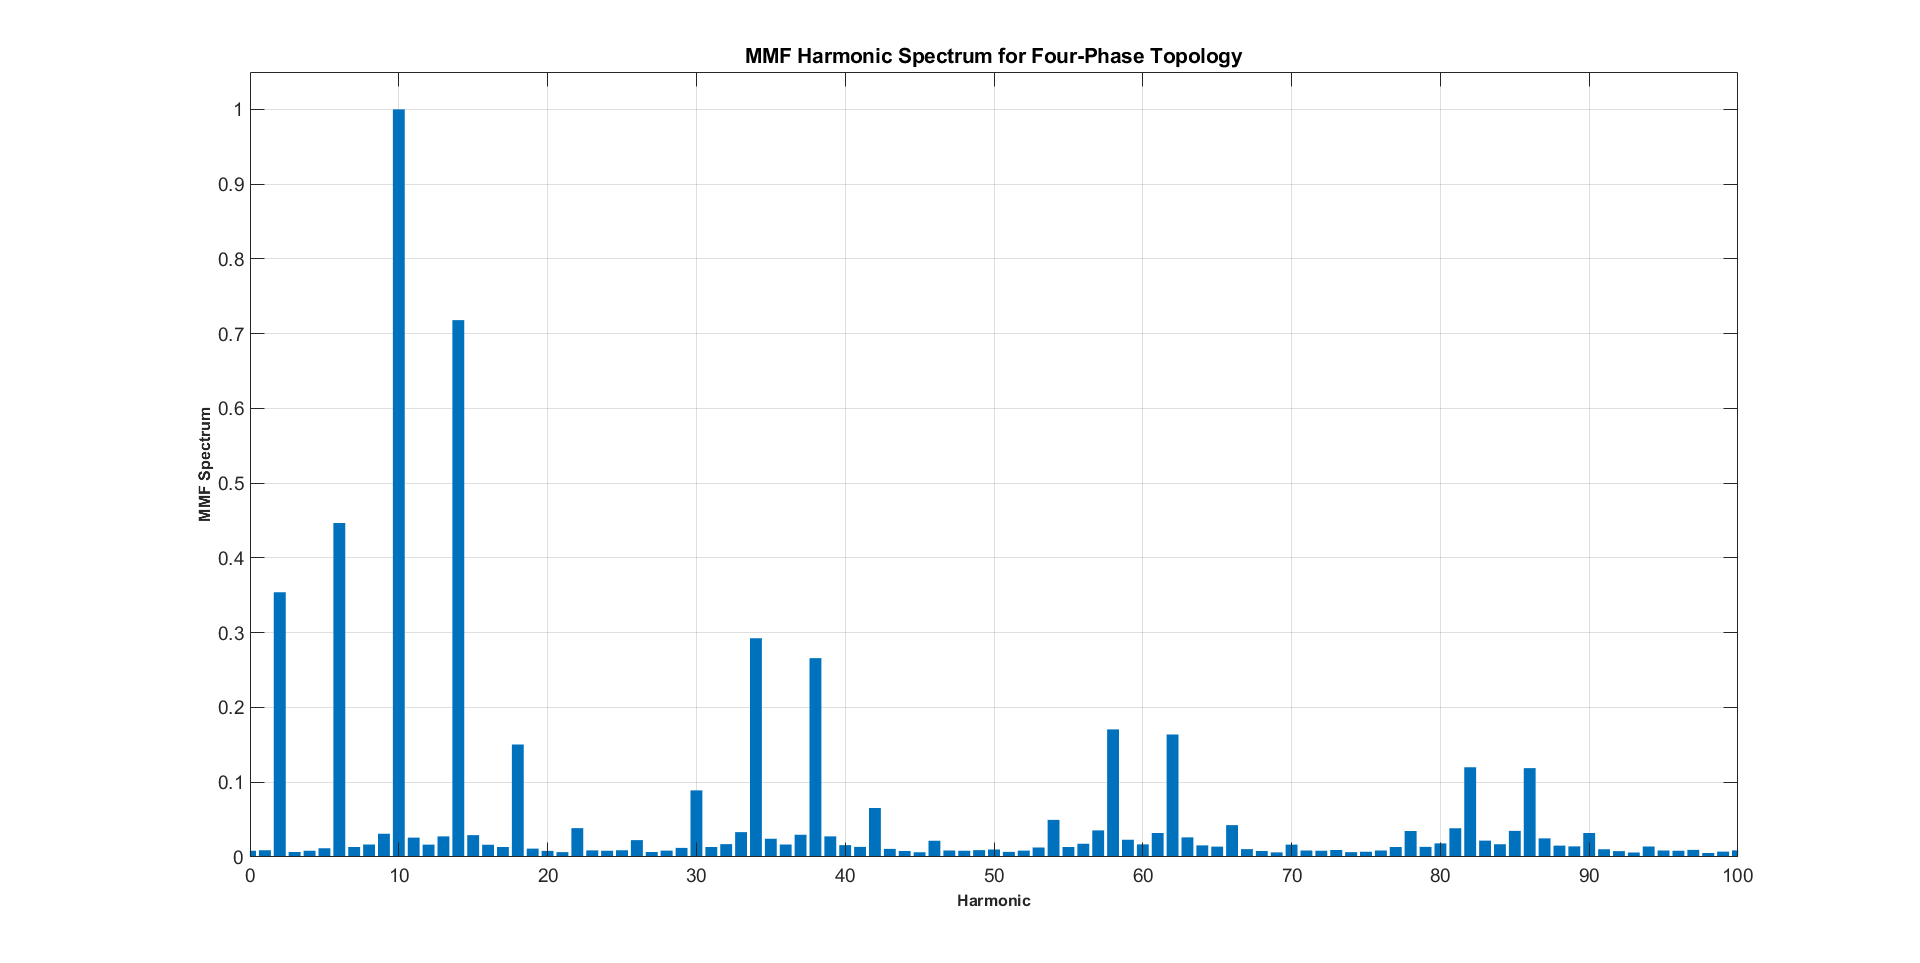
\includegraphics[width=\linewidth]{mmf_harm_4ph.png}
    \caption{Four-Phase}
    \label{fig:4phmmf}    
\end{subfigure}
\begin{subfigure}[b]{0.33\textwidth}
    \centering
    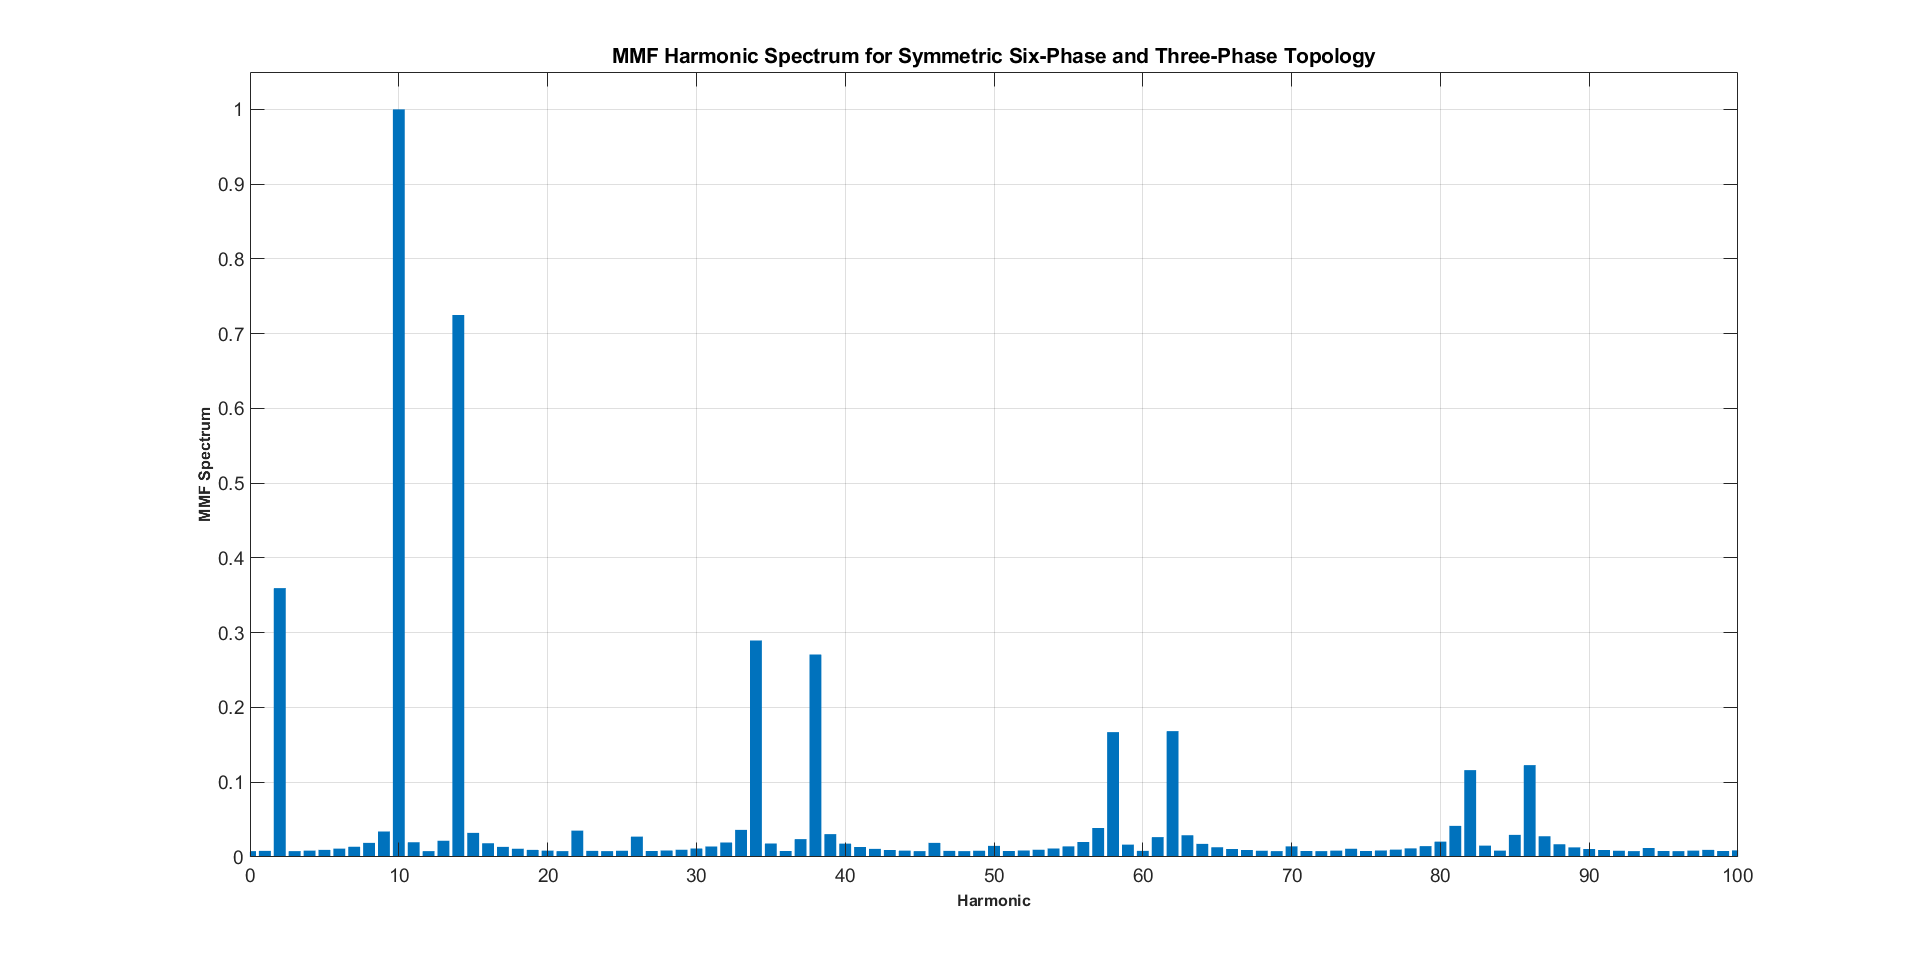
\includegraphics[width=\linewidth]{mmf_harm_sym.png}
    \caption{Symmetric Six-Phase}
    \label{fig:s6phmmf}    
\end{subfigure}
\begin{subfigure}[b]{0.33\textwidth}
    \centering
    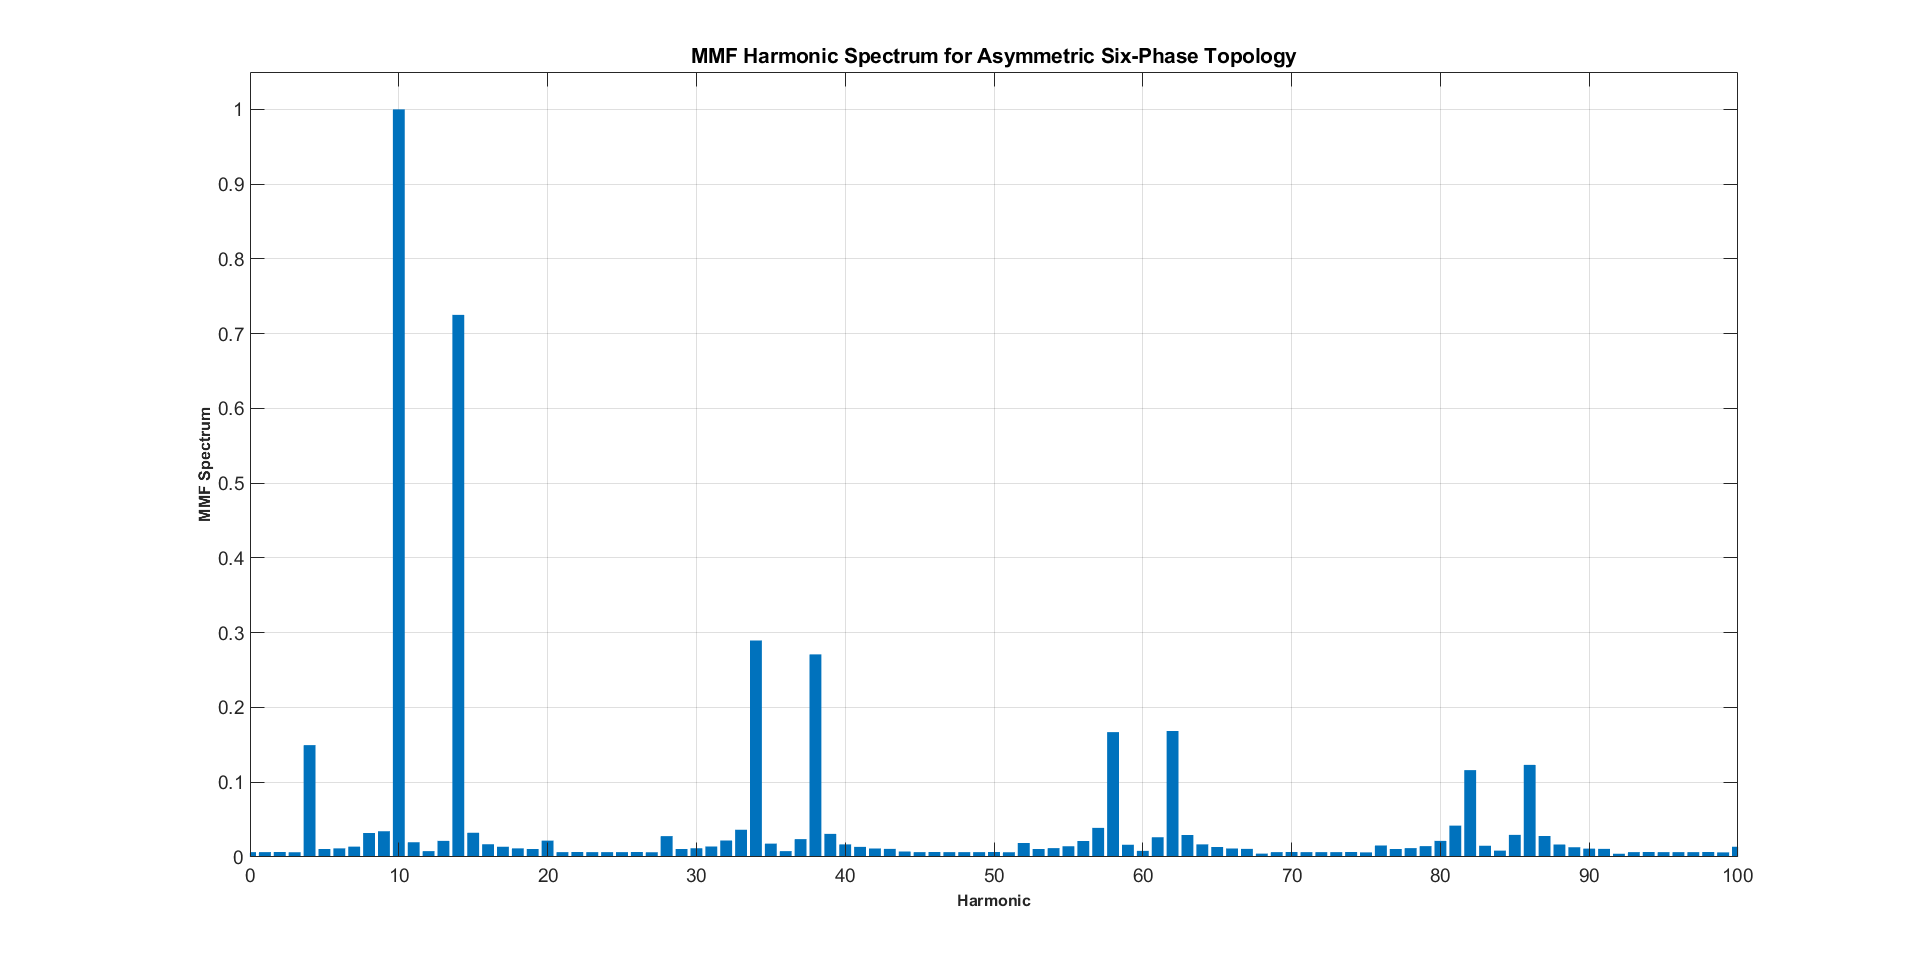
\includegraphics[width=\linewidth]{mmf_harm_asym.png}
    \caption{Asymmetric Six-Phase}
    \label{fig:as6phmmf}    
\end{subfigure}
 \caption{MMF Harmonic Spectrums}
\end{figure}


\section{\normalsize\textbf{Comparison of Different Topologies}}
\subsection{\normalsize\textbf{Redundancy}}
As aforementioned in the previous section, a three-phase machine is unable to operate properly under an OCF condition, as two phases cannot produce a rotating MMF.Yet, multiphase machines and machines with redundant phase legs may still maintain proper operation with certain manipulations. Accordingly, for the three-phase four module topology, OC failure of a single phase results in turning off one module completely. In this case, output power is decreased by 25\%. Although symmetric six-phase topology has the same magnetic equivalent circuit with three-phase four module, neutral node connection between two modules in this topology provides multiphase operation opportunity and as a result, completely turning off one module is not necessary. Similar advantages are also applicable for four-phase and asymmetric six-phase cases. On the other hand, decreasing the module number by half brings out other drawbacks. In a controller fault situation, which affects one module of the driver, decreases the motor output power to half, where it only decreases a quarter in initially proposed three-phase four module IMMD structure.

\subsection{\normalsize\textbf{Torque Ripple}}

\subsection{\normalsize\textbf{Open Circuit Failure (OCF) Responses and Recovery}}

\subsection{\normalsize\textbf{Overall Comparison}}
Torque ripple
eff?
??
Fault tolerance
Redundancy yüzdesi, normal operation, one phase open fault durumunda olacaklar, ilk IMMD topolojisiyle kıyaslanması, fault durumunda akımların, torque ripple ve average torque'un değişimi belirtilip karşılaştırılacak. Tablolanabilir. Akım vs gibi şeylerin simülasyonu genel olarak Simulink üzerinden yürüyecek. Tork için FEA karşılaştırması da eklenecek. Fault durumunda düzgün operate ettirmek için faz açısı kaydırma mevzularına girilecek. Genel olarak karşılaştırma bu değşik modül ve faz sayılı topolojilerin redundancy karşılaştırması üzerinden yürüyecek. 

\begin{table*}[ht!]
 \caption{Comparison of Different Topologies}
\label{kd}
\begin{tabularx}{\textwidth}{@{}l*{10}{C}c@{}}
\toprule
Advantages      & Three-Phase  & Four-Phase & Symmetric Six-Phase & Asymmetric Six-Phase \\ 
\midrule
Redundancy Factor    & lol    & lol    & lol   & lol \\ 
Overcurrent in OCF   & xd      & xd  & xd    & xd \\ 
Inductance Balance  &  asd &   asd&    asd&  asd\\
Torque Ripple  & menemene  & soğanları   & doğradım   & evet  \\
MMF Harmonics  & medium    & high  & medium  & low  \\ 
Interleaving Opportunity  & evet  & şöyle   & şarkımızı   & söyleyelim  \\


\bottomrule
\end{tabularx}
\end{table*}
\section{\normalsize\textbf{Conclusions}}
Toparlama. Ne yapmıştık bugün. Ne kattık biz bu çalışmayla. Experimental sonuç verecek miyiz full paperda, neleri ekleriz full papera onları yazarız.

\AtNextBibliography{\tiny}
\printbibliography

\end{document}
